In this report, we will explain what the Level Set method is and what
its applications are. Furthermore, we will provide code examples of
how to implement the mathematical formulas needed to create a Level
Set framework.

The Level Set method is a numerical technique used to transform
surfaces in $d$ dimensions. Transform means that we move the surface. The surfaces are transformed by solving a
partial differential equation(PDE) dependant on a time factor.

The level set at its most simple representation is a static
datastructure. It can be represented as a topographic map indicating
heights in a region, displayed in figure \vref{fig:isocontour-2d} or
it can be seen as a meteorological map, displaying weather data like
pressure. 
In figure \vref{fig:heightmap} we see two figures describing a 2-d and 3-d view of an island. Figure \vref{fig:isocontour-2d} describes an isocontour map of heights where the color indicates the height of each point. The brighter the color the higher the point. Figure \vref{fig:isocontour-3d} shows the corresponding 3d view.  

\begin{figure}[h]
\begin{center}
  \subfloat[2D view of an elevation isocontour map]{
    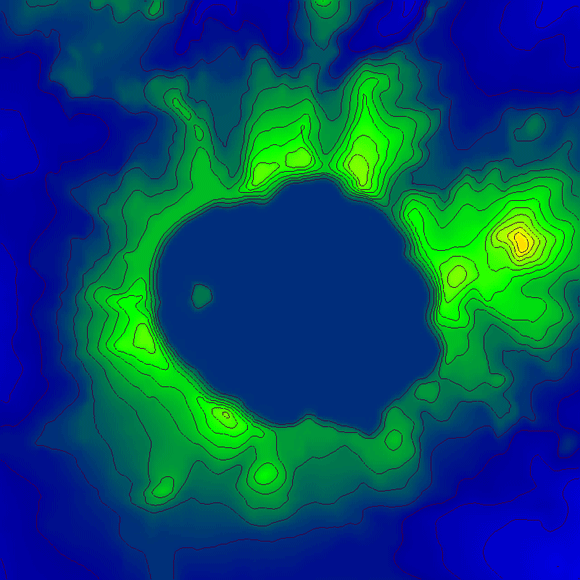
\includegraphics[width=0.5\textwidth]{imgs/226171_226171.png}
    \label{fig:isocontour-2d}
  }
  \subfloat[3D view of figure \ref{fig:isocontour-2d}]{
    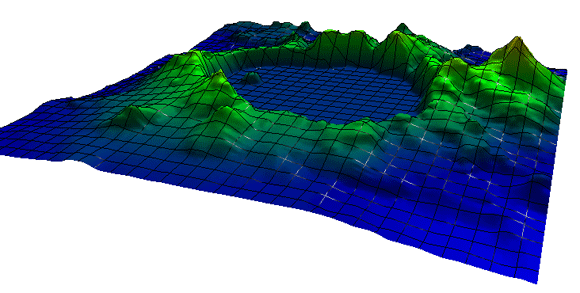
\includegraphics[width=0.5\textwidth]{imgs/226170_226170.png}
    \label{fig:isocontour-3d}
  }
\end{center}
\caption{Illustrations of heightmap, from: Intel Array Visualizer Gallery}
\label{fig:heightmap}
\end{figure}

%Intel Array Visualizer Gallery
%website\footnote{\url{http://www.intel.com/cd/software/products/apac/zho/perflib/226296.htm}}
\todoHave{husk reference}

%\image{hoejdekort.png}{0.25}{A topographic map indicating heights in the vermont region.}{introduction:fig:hoejdekort}

\section*{Signed distance function - $\phi$}

We would like a suitable way to indicate whether we are inside or outside the isocontour. 

We use an implicit representation of the surface. The Level Set method
can use implicit functions which means that the function is defined in
the entire plane and not only on the object.

The function $\phi(x,y)$ is a signed distance function in all of
$\mathbb{R}^{n}$, in our case $\mathbb{R}^{2}$. A signed distance
function $\phi$ is a function that given a point on the plane, returns
the distance to the surface. We have that $\phi(x,y) > 0$ if we are
outside the object and $\phi(x,y) < 0$ when we are inside the object.
And last, when $\phi(x,y) = 0$ we are on the interface or iso-surface.
The iso-surface separates the inside and outside.  Besides indicating
whether we are inside or outside an object, it also indicates how far
we are from the closest point on the iso-surface which is quite
handy. For a picture of the above, see figure
\vref{introduction:fig:implicitfunction}.

\image{phi.png}{0.3}{The figure is borrowed from
\cit{osher2002level}. A implicit function, defined in all of
$\mathbb{R}^{2}$. We see that when we are inside the object then
$\phi$ is less than zero, larger when we are outside and zero on the
interface.}{introduction:fig:implicitfunction}

%% Example - Circle

\subsection*{Example}

A simple example is to consider a circle and its equation:
\begin{equation*} 
  x^{2} + y^{2} = r^{2}
\end{equation*}

It is defined in all points in $\mathbb{R}^{2}$ and is an example of
an implicit function. Given a specific radius $r$, the equation of a
circle defines an isocontour. If $r = 5$, then the isovalue is $c =
5^{2} = 25$. For all the points $(x,y)$ that evaluate to 25 gives us
the isosurface. If the value is smaller then it is inside the surface,
and outside when the value is greater. See figure
\vref{introduction:fig:cartesiangrid}.


\section*{Cartesian grid}
\begin{comment} Finite memory -> descritization of plane -> cartesian
grid is used.
\end{comment}

Since a computer has finite memory we need to come up with a way to
store our representation. A simple way to do this that scale in the
number of dimensions is to partition the region into a grid where each
square is of equal size.

\begin{figure}[htb] \centering
    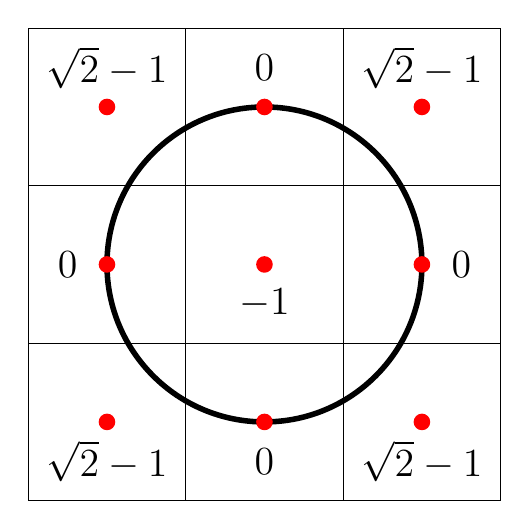
\begin{tikzpicture}[font=\Large]
    \draw (0,0) rectangle +(2,2)
    +(1,0.5) node {$-1$};    
    \draw (0,2) rectangle +(2,2)
    +(1,1.5) node {$0$};
    \draw (2,0) rectangle +(2,2)
    +(1.5,1) node {$0$};
    \draw (0,-2) rectangle +(2,2)
    +(1,0.5) node {$0$};
    \draw (-2,0) rectangle +(2,2)
    +(0.5,1) node {$0$};
    \draw (2,2) rectangle +(2,2)
    +(1,1.5) node {$\sqrt{2}-1$};
    \draw (2,-2) rectangle +(2,2)
    +(1,0.5) node {$\sqrt{2}-1$};
    \draw (-2,2) rectangle +(2,2)
    +(1,1.5) node {$\sqrt{2}-1$};
    \draw (-2,-2) rectangle +(2,2)
    +(1,.5) node {$\sqrt{2}-1$};
    \draw[line width=2pt] (1,1) circle (2);
    \fill[shift={(1,1)},red]
    (0,0) circle (3pt)
    (2,0) circle (3pt)
    (0,2) circle (3pt)
    (-2,0) circle (3pt)
    (0,-2) circle (3pt)
    (-2,-2) circle (3pt)
    (2,-2) circle (3pt)
    (-2,2) circle (3pt)
    (2,2) circle (3pt)    
    ;
  \end{tikzpicture}
  \caption{Borrowed from \cit{JLTGK}. A circle, descritized into a
cartesian grid. The value in each cell is the $\phi$ value described
in this chapter.}
  \label{introduction:fig:cartesiangrid}
\end{figure}

In figure \vref{introduction:fig:cartesiangrid}, we see how a plane
has been descritized into a cartesian grid, showing a circle and the
values of $\phi$.

%% formulas

\section*{Solving the Level Set}\label{sec:intro:solve} 

\todoPtx{I own this!!}

If we want to move the level set, we have to iteratively solve a Partial
differential equation to make the surface move. We solve a partial
differential equation in all points $(x,y) | x,y \in
\mathbb{R}^{2}$. If we want to move the interface in the normal
direction we solve the following equation:

\begin{equation}
\phi_{t} + a|\nabla \phi| = 0
\end{equation}\label{eq:normMove}

where $\nabla \phi = (\dfrac{\partial \phi}{\partial x},
\dfrac{\partial \phi}{\partial y})$ and $a$ can be of either sign.

When $a > 0$ the interface moves in the normal direction and when $a <
0$ it moves in the opposite direction of the normal.


\section*{Applications}

The advantages are that since we discretize the surface into a
cartesian grid, we can do numerical computations without having to
parameterize the objects. Another advantage is that the level set
method makes it easy to work on geometry that change topology over
time.


%% applications.  So why do we want to use the level set method? A
simple example is to consider an object that splits in two or two
objects merging into one. If we did not use the level set method, we
would have to explicitely represent the two new objects, where in the
level set case we get this for free do to the implicit representation.

\todoPtx{måske lidt flere anvendelsesmuligheder (lysberegninger her!)}

\newpage

\section*{Outline of the report}\todoPtx{Denne er på en side for sige
selv, så vref ikke crasher}

In chapter \vref{chap:sdf}, we give an in depth look on the signed
distance function, describe what kinds of mathematical operations we
have in our toolbox and describe the important reinitialize function,
section \vref{sec:reinitialize}.

In chapter \vref{chap:extensions}, we look at extension that can be
made to the basic level set implementation that we have done. In
section \vref{sec:segmentation}, we look at how to implement
segmentation algorithms which can be used in mediacal imaging. In
section \vref{sec:fluid}, we implement a fluid solver for computer
graphics using the level set method. And finally, in section
\vref{sec:imagereconstruction} \todoHave{Skal CPVC's afsnit være med i
den endelige rapport? (have)} we use the level set to do computations
on images.



%%% Local Variables: 
%%% mode: latex 
%%% mode: auto-fill 
%%% TeX-PDF-mode: t 
%%% TeX-master: "../master.tex" 
%%% End:

